\documentclass[11pt]{article}
\usepackage[margin=1in]{geometry}
\usepackage[T1]{fontenc}
\usepackage[utf8]{inputenc}
\usepackage{lmodern}
\usepackage{graphicx}
\usepackage{booktabs}
\usepackage{tabularx}
\usepackage{longtable}
\usepackage{calc}
\usepackage{float}
\usepackage{xcolor}
\usepackage{amsmath,amssymb}
\usepackage[numbers,sort&compress]{natbib}
\usepackage[hidelinks]{hyperref}
\providecommand{\doi}[1]{\href{https://doi.org/#1}{https://doi.org/#1}}
\setlength{\emergencystretch}{3em}
\setlength{\parindent}{1.5em}
\setlength{\parskip}{0.25em}
\linespread{1.18}
\sloppy
\renewcommand{\refname}{References}
\providecommand{\tightlist}{\setlength{\itemsep}{0pt}\setlength{\parskip}{0pt}}
\providecommand{\real}[1]{#1}
\title{Operator identity and out-of-user generalization in automated surgical skill assessment: a multi-dataset evaluation}
\author{Hamilton Jeong\textsuperscript{1,*}, Zaid Elnasser\textsuperscript{1},
Laurienne Jeong\textsuperscript{1}, Bhumika Iroji\textsuperscript{2},\\
Su\'elia de Siqueira Rodrigues Fleury Rosa\textsuperscript{3}\\[0.75em]
\small \textsuperscript{1}College of Agriculture and Life Sciences, Cornell University,\\
\small 215 Garden Avenue, Ithaca, NY 14850, USA\\
\small \textsuperscript{2}College of Engineering, Cornell University, 313 Campus Road, Ithaca, NY 14850, USA\\
\small \textsuperscript{3}Meinig School of Biomedical Engineering, Cornell University,\\
\small 237 Tower Road, Ithaca, NY 14850, USA\\[0.5em]
\small \textsuperscript{*}Corresponding author: \href{mailto:hhj22@cornell.edu}{hhj22@cornell.edu}}
\date{}
\begin{document}
\maketitle
\begin{abstract}
\textbf{Purpose:} Repeated recordings from the same operator can permit surgical-performance models to use operator-specific motion patterns. We tested whether operator identity was recoverable from surgical kinematics and whether suppressing that information improved prediction for unseen operators.

\textbf{Methods:} We retrospectively analyzed 2,501 dry-lab trials representing 92 dataset-participants from JIGSAWS, ROSMA, BGU-PatCut, and BGU-SKILLS. Outcomes were expert-rated Global Rating Scale, observed task errors, and image-derived cutting error; BGU-SKILLS contributed to identity analysis only. We compared same-participant with held-out-participant evaluation, used fresh linear and random-forest identity probes and JIGSAWS label permutations, and evaluated duration removal, duration residualization, linear identity-subspace projection (I3), and adversarial suppression (I4). Intervals used 2,000 participant bootstrap replicates.

\textbf{Results:} Unsuppressed identity accuracy exceeded its record-wise permutation null in all ten dataset-task groups (linear 0.228--0.944; nonlinear 0.381--0.844; each empirical $p=0.0196$). JIGSAWS participant-wise permutations retained substantially more same-participant skill accuracy than record-wise permutations (median differences 0.444--0.538; each $p=0.004975$). I3 reduced fresh linear identity accuracy by 0.184 (95\% interval 0.151--0.215) and nonlinear accuracy by 0.138 (0.098--0.175); I4 failed the prespecified two-probe rule. Held-out-participant standardized mean absolute error favored I3 in one of seven tasks and the unsuppressed model in six; six intervals crossed zero.

\textbf{Conclusion:} Identity was recoverable and targeted projection reduced tested identity recovery, but suppression did not consistently improve unseen-operator prediction. Identity diagnostics and held-out-user utility should be evaluated separately.
\end{abstract}

\noindent\textbf{Keywords:} surgical skill assessment; operator identity; out-of-user validation; domain generalization; kinematics; representation learning

\noindent\textbf{Total word count:} 4,245
\section{Introduction}\label{introduction}

Automated assessment could make surgical-training feedback more
reproducible, but studies often contain small cohorts, repeated trials
from each operator, and heterogeneous targets \citep{Lam2022}. Shared
resources such as JIGSAWS support comparison across methods
\citep{Ahmidi2017}, yet a record-wise split can place trials from one
person in both training and testing. A model may then exploit stable
operator-specific motion patterns rather than information that transfers
to a new operator, a form of shortcut learning \citep{Geirhos2020}.
Claims about unseen users therefore require participant-held-out
evaluation.

A same-participant versus held-out-participant performance gap reveals
protocol sensitivity, while an identity probe tests whether a
representation contains operator-identifying information. Neither proves
that the outcome model uses identity. For person-constant labels,
participant-wise permutation preserves identity-to-label lookup after
destroying the original label assignment, whereas record-wise
permutation breaks both.

An earlier unpublished JIGSAWS-only manuscript and software repository
from this project (https://github.com/hahnyu/surgical-skill) analyzed
the same 103 JIGSAWS trials. The present JIGSAWS component is therefore
a replication and mechanistic extension, not independent validation.
This study adds ROSMA, BGU-SKILLS, and BGU-PatCut; a harmonized
representation; prespecified identity-suppression interventions; fresh
probes; negative controls; and participant-level inference.

We asked whether operator identity was recoverable across
surgical-training datasets and whether verified suppression improved
prediction for an unseen operator. We expected identity recovery above
empirical nulls and participant-wise JIGSAWS permutations to retain more
same-participant classification than record-wise permutations. We
evaluated utility only after requiring suppression to reduce both fresh
linear and nonlinear identity probes.

\section{Methods}\label{methods}

\subsection{Study design, datasets, and
outcomes}\label{study-design-datasets-and-outcomes}

This retrospective benchmark followed a protocol frozen before
predictive modeling (\texttt{protocol-v1}, 21 September 2026). Trials
remained intact within folds, analyses were task specific, and the
participant was the independent unit for uncertainty. The analysis
included 2,501 dry-lab trials representing 92 dataset-participants
across four distinct cohorts. JIGSAWS contributed 103 trials and
expert-rated Global Rating Scale (GRS); its self-declared experience
class was used only for a person-level diagnostic. ROSMA contributed 206
trials with observed task-error counts. BGU-PatCut contributed 1,254
trials with image-derived total cutting error. BGU-SKILLS contributed
938 trials to identity and longitudinal robustness analyses because its
available performance metrics were derived from the planned kinematic
predictors. Source provenance and detailed inclusion rules are reported
in Online Resource 1
\citep{RivasBlanco2023, ROSMAData2022, SharonPatCut2024, PatCutData2024, Sharon2025, BGUSkillsData2025}.

\subsection{Features, validation, and
models}\label{features-validation-and-models}

Task windows followed source annotations. The harmonized representation
contained 41 available variables spanning duration, per-arm sample count
and rate, path length, speed, acceleration, jerk, idle fraction,
workspace, missing-data gaps, gripper summaries where available,
bimanual speed correlation, and path-length asymmetry. Imputation,
scaling, model selection, and every learned transformation used
training-fold data only.

Same-participant folds retained each participant on both sides;
held-out-participant folds withheld complete participants. Inner
validation matched the outer generalization unit. Continuous outcomes
used training-mean, duration-only ridge, and all-feature ridge models
with nested penalty selection. JIGSAWS person-level classification used
majority, duration-only multinomial-logistic, and all-feature
multinomial-logistic models. All predictions were out of fold.

\subsection{Identity diagnostics and
interventions}\label{identity-diagnostics-and-interventions}

Identity probes predicted participant labels with nested multinomial
logistic regression and random forests; balanced accuracy was averaged
by participant. Fifty record-wise identity-label permutations supplied
each dataset-task null. For JIGSAWS experience classification, 200
paired participant-wise and record-wise permutations were evaluated
under same-participant folds.

I0 retained all features. I1 removed duration equivalents, and I2
residualized remaining features on duration. I3 fitted a regularized
participant classifier within each training fold and projected out
selected coefficient-span directions, following linear guarding
principles \citep{Ravfogel2020}. A dimension-matched random projection
served as a control. I4 used an eight-unit latent multilayer perceptron
with a gradient-reversal identity head \citep{Ganin2016}, plus capacity
and shuffled-label controls. After freezing each representation, new
linear and nonlinear probes tested identity recovery. The primary
intervention had to reduce both probes; I4 was considered first, with I3
versus I0 prespecified if I4 failed.

\subsection{Estimands and inference}\label{estimands-and-inference}

The primary utility estimand was participant-average
held-out-participant MAE(I3) minus MAE(I0); negative values favor I3.
Trial differences were also standardized by the outcome standard
deviation estimated without the outer test fold. We report native-unit
effects because outcomes represented different constructs and did not
pool tasks. Percentile intervals used 2,000 participant bootstrap
replicates. Permutation tests used plus-one empirical \emph{p} values.
Leave-one-participant estimates assessed influence. Locked artifact
hashes, complete hyperparameters, deviations, and reproducibility
controls are in Online Resource 1; reporting follows an adapted
TRIPOD+AI checklist \citep{Collins2024}.

\section{Results}\label{results}

\subsection{Feasibility and target
audit}\label{feasibility-and-target-audit}

All datasets contained repeated trials and stable participant keys.
JIGSAWS supplied the only expert-rated outcome; ROSMA errors and
BGU-PatCut cutting error were retained as narrower task-performance
outcomes. BGU-SKILLS was not relabeled with a kinematics-derived
outcome.

\begin{figure}[H]
\centering
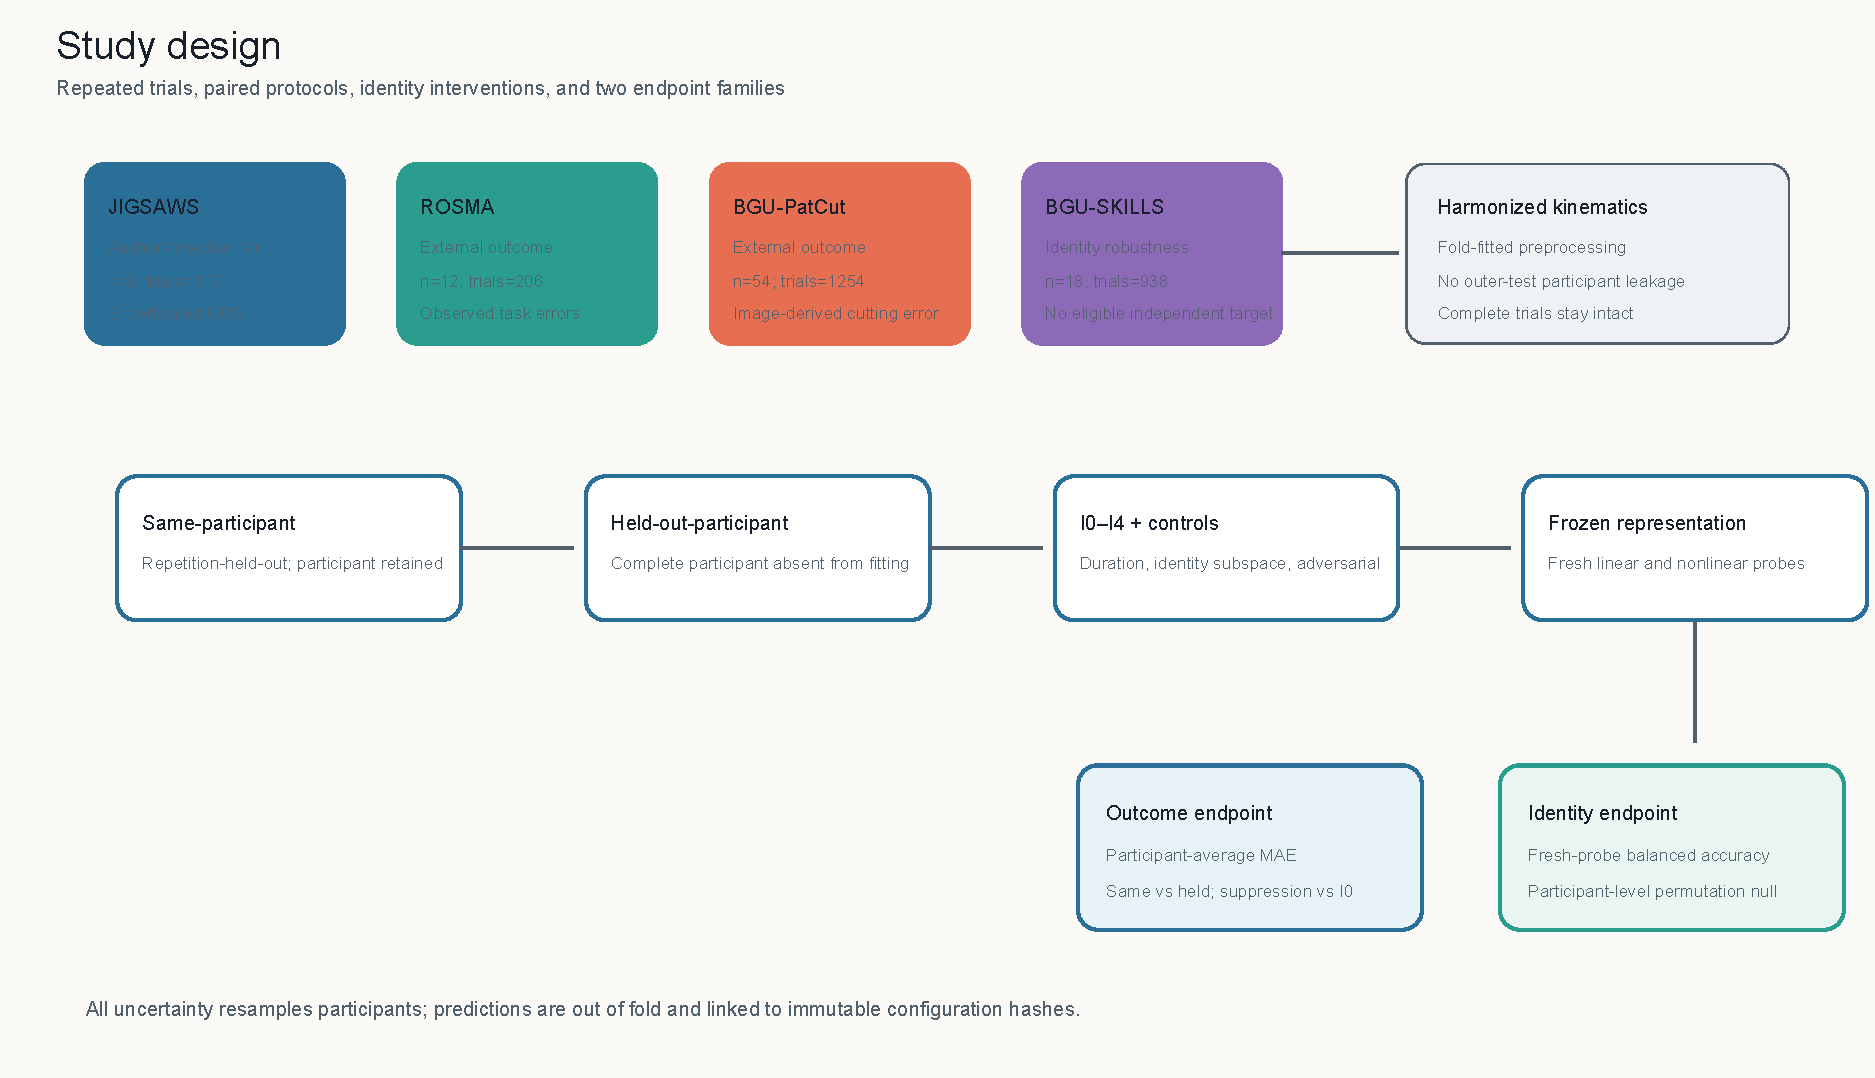
\includegraphics[width=0.96\textwidth]{figures/Fig1.pdf}
\caption{Study design, datasets, validation protocols, identity diagnostics, interventions, and locked inference.}
\label{fig:phase5-1}
\end{figure}

\begin{table}[H]
\centering
\caption{Datasets, cohorts, outcomes, and analysis roles. Participant counts are dataset-specific and are not linked across cohorts.}
\label{tab:datasets}
\small
\begin{tabularx}{\textwidth}{@{}lXrrX@{}}
\toprule
Dataset & Tasks & Trials & Participants & Retained role/outcome \\
\midrule
JIGSAWS & Knot tying; needle passing; suturing & 103 & 8 overall & Expert-rated GRS; person-level mechanism \\
ROSMA & Pea on a peg; post and sleeve; wire chaser I & 206 & 12 & Observed task-specific errors \\
BGU-SKILLS & Knot tying; ring tower transfer; suturing & 938 & 18 & Identity and longitudinal robustness only \\
BGU-PatCut & Pattern cutting & 1,254 & 54 & Image-derived total cutting error \\
\bottomrule
\end{tabularx}
\end{table}

\begin{table}[H]
\centering
\caption{Harmonized kinematic feature families. Forty-one variables were available after source-specific matching. All transforms were fitted within training folds.}
\label{tab:features}
\small
\begin{tabularx}{\textwidth}{@{}lclX@{}}
\toprule
Family & Count & Availability & Contents \\
\midrule
Cross-arm/time & 3 & All datasets & Duration, bimanual speed correlation, path-length asymmetry \\
Instrument arm 1 & 19 & All core features & Sample count/rate; path length; speed, acceleration, jerk; idle fraction; workspace; gaps; gripper summaries \\
Instrument arm 2 & 19 & All core features & Same summaries as arm 1 \\
Gripper subset & 8 total & Not present in ROSMA & Mean, SD, range, and total variation for each arm \\
\bottomrule
\end{tabularx}
\end{table}

\subsection{Protocol gap}\label{protocol-gap}

Figure 1 summarizes the study flow. Table 1 documents the analyzed
cohorts, and Table 2 lists the harmonized feature families.

Held-out-participant minus same-participant standardized ridge MAE was
positive in six of seven eligible tasks (Figure 2). JIGSAWS person-level
same-participant versus held-out-participant accuracy was 0.917 versus
0.444 for knot tying, 1.000 versus 0.464 for needle passing, and 0.872
versus 0.462 for suturing. Participant-average gaps were +0.419 (95\%
interval 0.063--0.775), +0.479 (0.214--0.757), and +0.400
(0.150--0.675).

\begin{figure}[H]
\centering
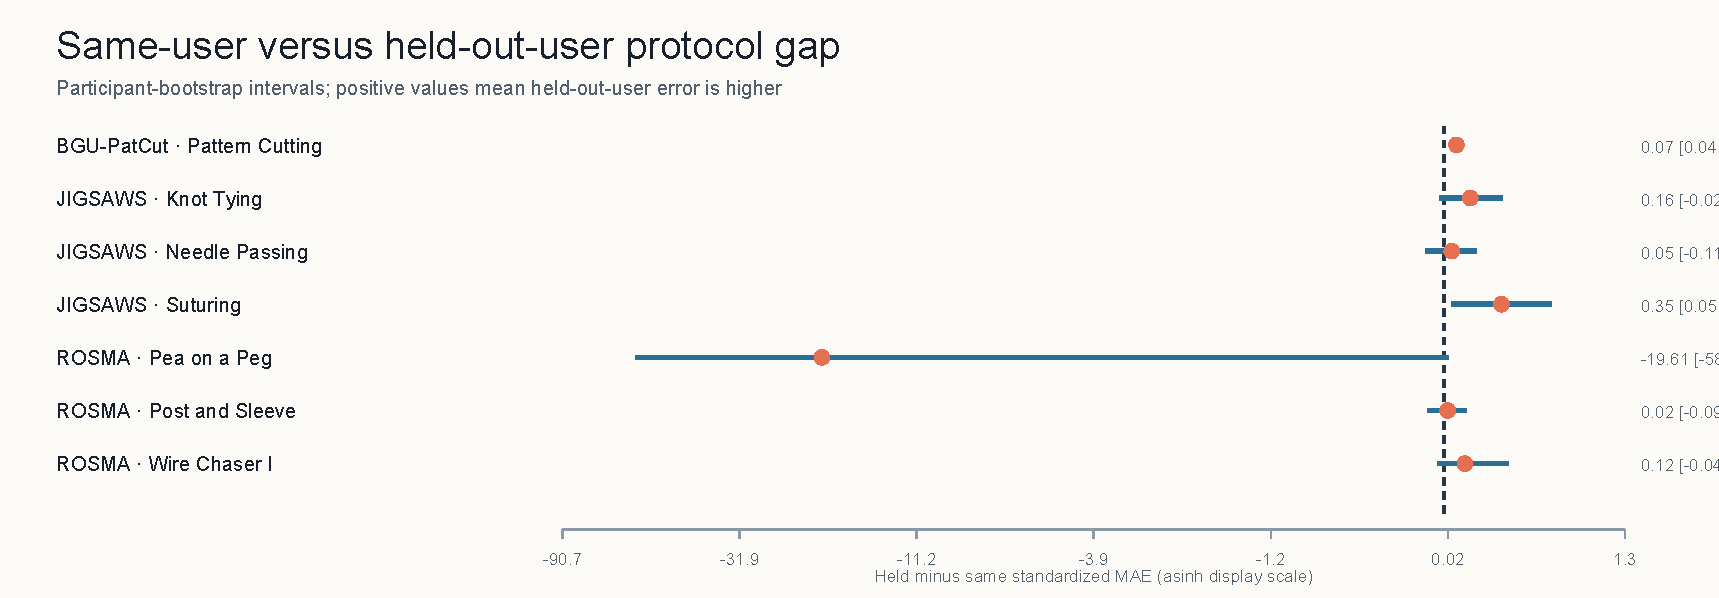
\includegraphics[width=0.96\textwidth]{figures/Fig2.pdf}
\caption{Standardized protocol gap for ridge prediction. Positive values indicate less favorable held-out-participant than same-participant error.}
\label{fig:phase5-2}
\end{figure}

\begin{table}[H]
\centering
\caption{Participant-average ridge mean absolute error under same-participant and held-out-participant evaluation. Values remain in each dataset's native outcome units.}
\label{tab:baselines}
\small
\begin{tabular}{@{}llrr@{}}
\toprule
Dataset & Task & Same participant & Held-out participant \\
\midrule
BGU-PatCut & Pattern Cutting & 9,231.214 & 10,440.406 \\
JIGSAWS & Knot Tying & 2.735 & 3.505 \\
JIGSAWS & Needle Passing & 3.029 & 3.202 \\
JIGSAWS & Suturing & 3.246 & 4.968 \\
ROSMA & Pea on a Peg & 21.120 & 6.475 \\
ROSMA & Post and Sleeve & 0.433 & 0.443 \\
ROSMA & Wire Chaser I & 0.444 & 0.518 \\
\bottomrule
\end{tabular}
\end{table}

\subsection{Identity recovery and formal
nulls}\label{identity-recovery-and-formal-nulls}

Table 3 reports the same-participant and held-out-participant baseline
errors used to frame the protocol comparison.

Identity was recoverable in every dataset-task group (Figure 3; Table
4). Linear balanced accuracy ranged from 0.228 to 0.944 and nonlinear
accuracy from 0.381 to 0.844; every full-feature probe exceeded its
50-permutation record-wise null (each empirical \emph{p}=0.0196).
Duration-only accuracy ranged from 0.056 to 0.225.

JIGSAWS participant-wise skill-label permutations retained substantially
more same-participant accuracy than record-wise permutations. Median
paired differences were +0.444 for knot tying, +0.536 for needle
passing, and +0.538 for suturing (each empirical \emph{p}=0.004975),
consistent with identity-compatible lookup.

\begin{figure}[H]
\centering
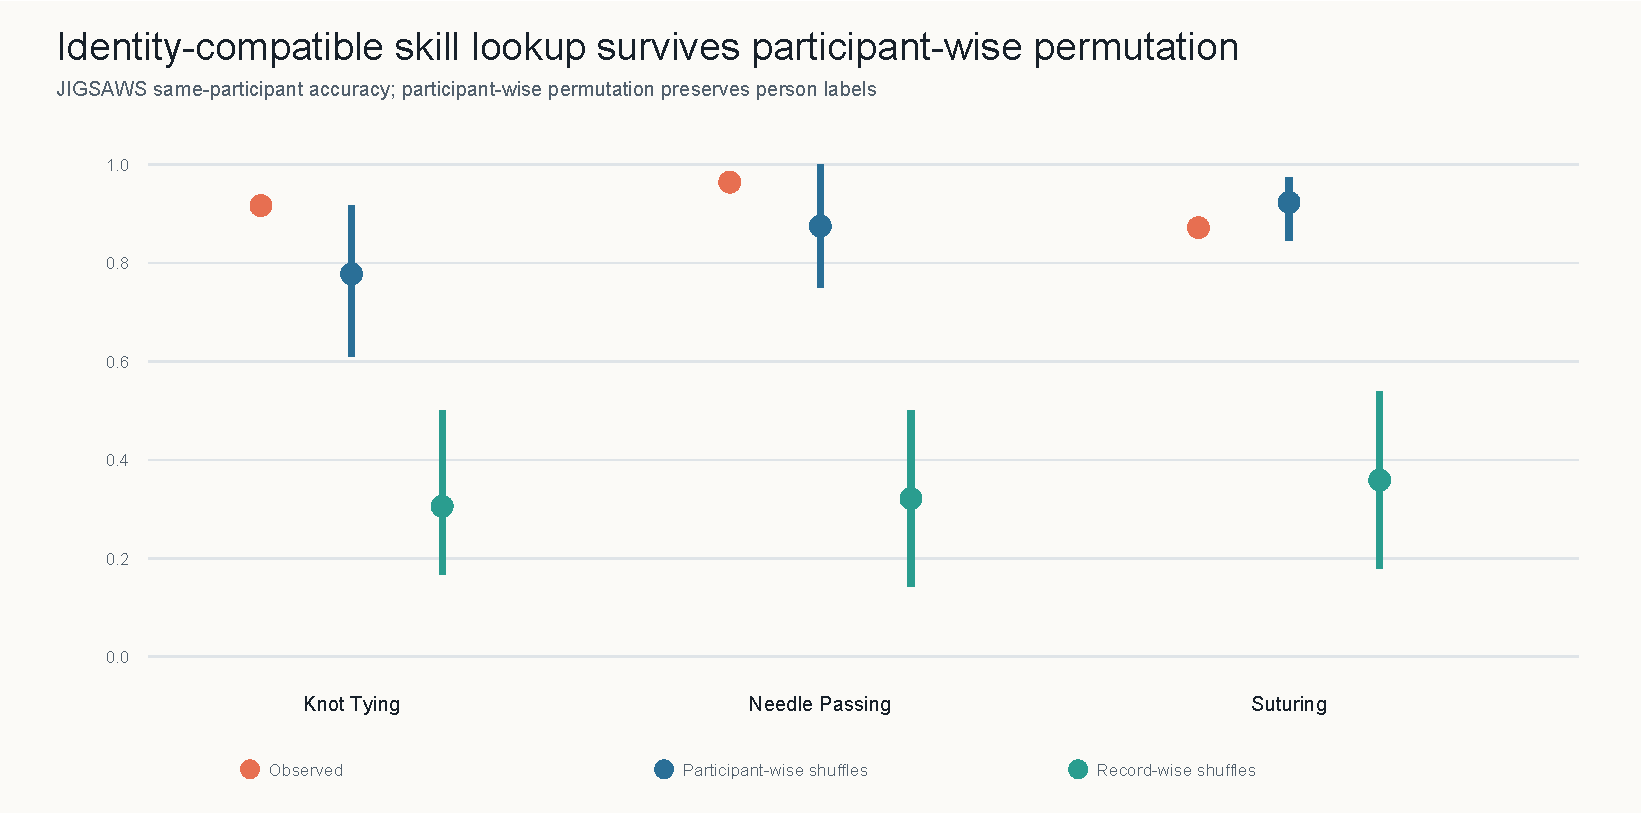
\includegraphics[width=0.96\textwidth]{figures/Fig3.pdf}
\caption{JIGSAWS same-participant person-level skill accuracy under observed labels and participant-wise versus record-wise permutations.}
\label{fig:phase5-3}
\end{figure}

\begin{table}[H]
\centering
\caption{Unsuppressed identity recovery. Balanced accuracy is participant averaged; the null is the median of 50 record-wise identity-label permutations.}
\label{tab:identity}
\scriptsize
\begin{tabular}{@{}llrrr@{}}
\toprule
Dataset & Task & Linear & Nonlinear & Null median \\
\midrule
JIGSAWS & Knot Tying & 0.869 & 0.827 & 0.084 \\
JIGSAWS & Needle Passing & 0.943 & 0.840 & 0.064 \\
JIGSAWS & Suturing & 0.944 & 0.844 & 0.075 \\
ROSMA & Pea on a Peg & 0.381 & 0.397 & 0.056 \\
ROSMA & Post and Sleeve & 0.446 & 0.381 & 0.062 \\
ROSMA & Wire Chaser I & 0.228 & 0.431 & 0.060 \\
BGU-SKILLS & Knot Tying & 0.530 & 0.393 & 0.051 \\
BGU-SKILLS & Ring Tower Transfer & 0.596 & 0.487 & 0.050 \\
BGU-SKILLS & Suturing & 0.762 & 0.618 & 0.049 \\
BGU-PatCut & Pattern Cutting & 0.834 & 0.750 & 0.016 \\
\bottomrule
\end{tabular}
\end{table}

\subsection{Intervention verification}\label{intervention-verification}

I4 reduced fresh linear identity accuracy by 0.048 (95\% interval
0.015--0.082) relative to its capacity control, but nonlinear accuracy
changed by -0.003 (-0.038 to +0.032); I4 therefore failed the two-probe
rule. I3 became primary. Relative to I0, I3 reduced linear balanced
accuracy by 0.184 (0.151--0.215) and nonlinear accuracy by 0.138
(0.098--0.175), averaging dataset-task groups equally (Figure 4).
Duration removal, duration residualization, and a dimension-matched
random projection did not reproduce this joint reduction.

\begin{figure}[H]
\centering
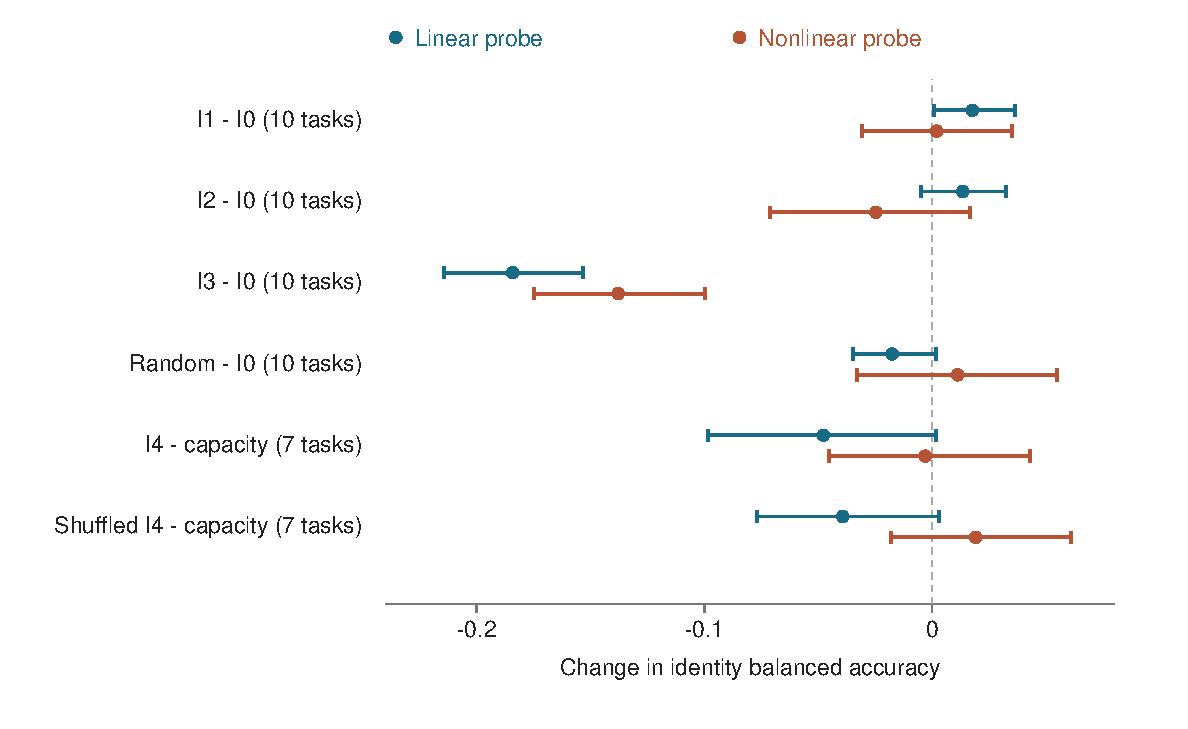
\includegraphics[width=0.84\textwidth]{figures/Fig4.pdf}
\caption{Relationship between fresh-probe identity change and held-out-participant task-utility change across interventions.}
\label{fig:phase5-4}
\end{figure}

\subsection{Held-out-participant
utility}\label{held-out-participant-utility}

Figure 4 relates intervention-associated identity changes to
held-out-participant utility changes.

Verified suppression did not consistently improve held-out-participant
prediction (Figure 5; Table 5). The standardized I3-minus-I0 MAE point
estimate favored I3 in one task and I0 in six; six of seven intervals
crossed zero. The wire-chaser estimate was +0.004 (0.000--0.011). The
ROSMA pea-on-a-peg standardized estimate was unstable because the
outcome was sparse and some outer-training standard deviations were
small. Native-unit estimates and all intervals are reported in Table 5.

\begin{figure}[H]
\centering
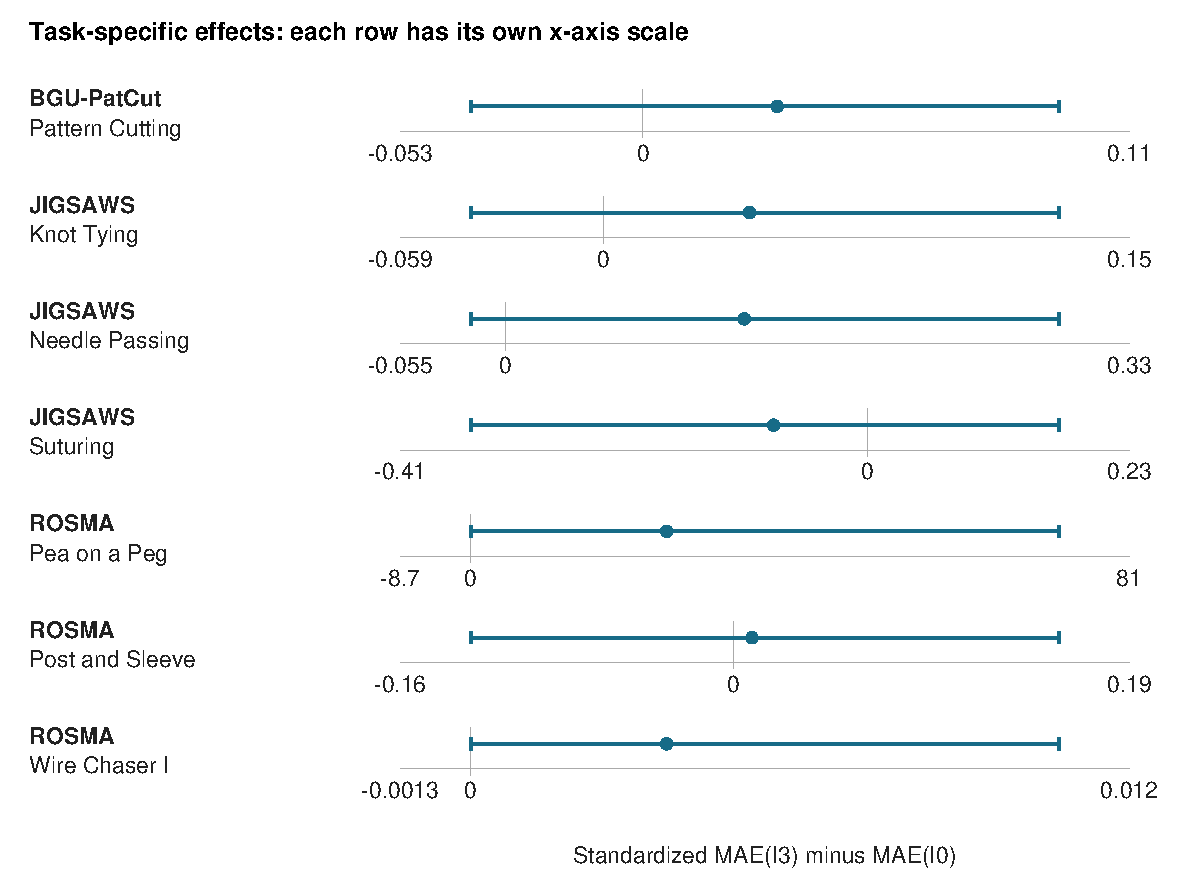
\includegraphics[width=0.72\textwidth]{figures/Fig5.pdf}
\caption{Task-specific held-out-participant standardized MAE differences for identity interventions and controls. Negative values favor the candidate intervention.}
\label{fig:phase5-5}
\end{figure}

\begin{table}[H]
\centering
\caption{Primary held-out-participant effects of I3 identity-subspace removal versus I0. Differences are MAE(I3) minus MAE(I0); negative values favor I3. Intervals resample participants.}
\label{tab:effects}
\scriptsize
\begin{tabularx}{\textwidth}{@{}lXrr@{}}
\toprule
Dataset & Task & Standardized difference [95\% interval] & Native difference [95\% interval] \\
\midrule
BGU-PatCut & Pattern Cutting & +0.029 [-0.038, +0.091] & +487.183 [-648.849, +1,613.362] \\
JIGSAWS & Knot Tying & +0.042 [-0.039, +0.132] & +0.205 [-0.195, +0.604] \\
JIGSAWS & Needle Passing & +0.125 [-0.018, +0.290] & +0.618 [-0.045, +1.400] \\
JIGSAWS & Suturing & -0.083 [-0.352, +0.170] & -0.401 [-1.757, +0.938] \\
ROSMA & Pea on a Peg & +24.141 [-0.019, +72.407] & +28.858 [-0.020, +86.539] \\
ROSMA & Post and Sleeve & +0.009 [-0.125, +0.154] & +0.005 [-0.072, +0.086] \\
ROSMA & Wire Chaser I & +0.004 [+0.000, +0.011] & +0.003 [0.000, +0.008] \\
\bottomrule
\end{tabularx}
\end{table}

\subsection{Same-participant skill and
robustness}\label{same-participant-skill-and-robustness}

For JIGSAWS person-level skill, I3 changed same-participant accuracy by
-0.025 (-0.075 to 0.000) for knot tying, 0.000 (0.000 to 0.000) for
needle passing, and +0.025 (-0.100 to +0.125) for suturing (Figure 6).
The expected consistent reduction was absent. Fresh nonlinear probes
also showed that confusing I4's training adversary did not establish
invariance. Influence, seed, fold, missingness, and hyperparameter
analyses are reported in Online Resource 1.

\begin{figure}[H]
\centering
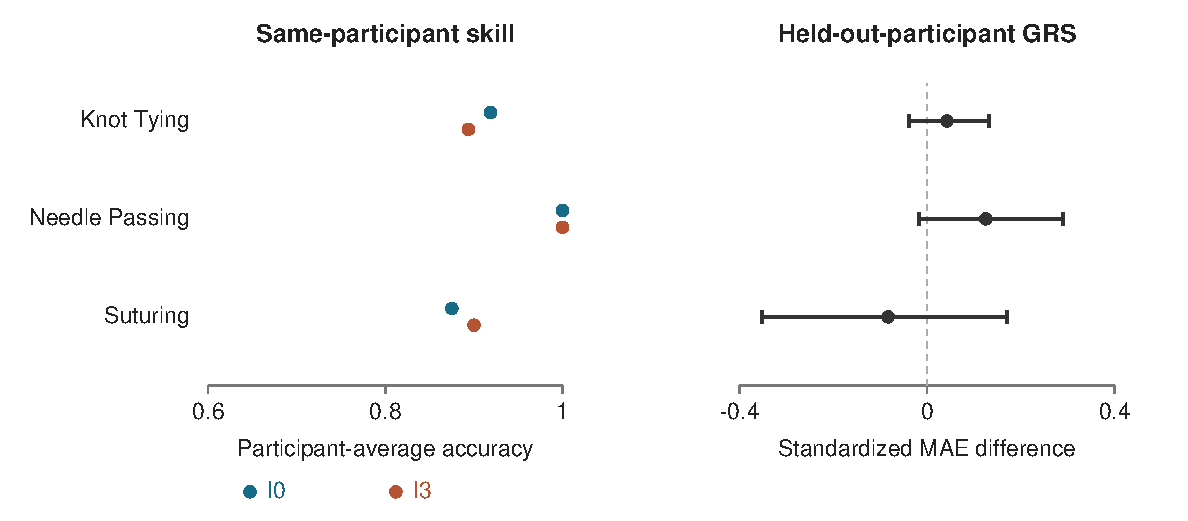
\includegraphics[width=0.96\textwidth]{figures/Fig6.pdf}
\caption{JIGSAWS mechanism summary: protocol gap, identity-compatible permutation behavior, probe verification, and same-participant skill effects.}
\label{fig:phase5-6}
\end{figure}

\section{Discussion}\label{discussion}

Operator identity was recoverable across four surgical-training
datasets, and JIGSAWS participant-wise permutations showed that
person-compatible structure could sustain same-participant
classification after the original experience assignments were destroyed.
Targeted linear projection reduced both fresh identity probes. This
verified reduction nevertheless did not consistently improve prediction
for unseen operators.

Protocol gaps and identity probes diagnose opportunities for shortcut
use; they do not show that an outcome model depends on identity.
Removing a learned identity subspace can also discard stable motion
components that predict performance. The task-specific estimates, which
favored I0 in six of seven tasks but mostly included both benefit and
harm, support neither a universal benefit nor a universal cost of
suppression. The I4 result further shows why a separately fitted
nonlinear probe and matched controls are needed: the training adversary
can be confused while identity remains decodable.

Held-out-participant evaluation should match claims about new users.
Same-participant results remain relevant for systems that personalize to
known trainees, but answer a different question. When suppression is
proposed, independent probes should verify it and held-out-user utility
should be measured rather than assumed.

\subsection{Limitations}\label{limitations}

Independent cohorts were small despite 2,501 trials: JIGSAWS had seven
or eight participants per task, ROSMA 12, and BGU-SKILLS 18. Most
intervals therefore permit effects in either direction, and no
equivalence margin was prespecified. Outcomes were heterogeneous: only
JIGSAWS GRS was expert rated; ROSMA errors and BGU-PatCut error measured
narrower constructs. All tasks were simulated or dry-lab exercises, so
the results do not establish clinical validity, educational benefit,
fairness, or patient outcomes.

Identity may encode stable skill, motor strategy, prior training, or
measurement artifacts; I3 removes selected linear directions and cannot
prove that all identity is absent. The harmonized summary representation
also differs from sequence or video models. Demographic attributes were
unavailable. No prospective cohort or deployment study was performed,
and one retained ROSMA trial with source coordinate spikes contributed
to unstable pea-on-a-peg estimates.

\section{Conclusion}\label{conclusion}

Operator identity was recoverable across all examined kinematic task
groups, and JIGSAWS same-participant skill classification retained
substantial accuracy under participant-wise label permutation. Linear
identity-subspace projection reduced identity recovery by fresh linear
and nonlinear probes, but did not consistently improve prediction for
unseen operators. Claims about generalization should therefore rest on
participant-held-out evaluation, while claims about invariance require
independent probes and task-utility tests.

\section{Supplementary information}\label{supplementary-information}

Online Resource 1 (\texttt{ESM\_1.pdf}): detailed dataset provenance,
preprocessing, fold construction, model specifications, intervention
definitions, inference, locked numerical results, robustness analyses,
deviations, and reproducibility controls.

\section{Statements and declarations}\label{statements-and-declarations}

\subsection{Ethics approval}\label{ethics-approval}

This study was a secondary analysis of previously collected,
de-identified research datasets. The investigators had no direct
identifiers, no access to any re-identification key, and no interaction
or intervention with participants. Under Cornell University guidance for
research involving existing or secondary de-identified data, this
activity does not constitute federally regulated human-participant
research and did not require further Cornell Institutional Review Board
review. The original dataset investigators were responsible for the
ethics approvals and consent procedures applicable to the source
studies.

\subsection{Consent to participate and consent for
publication}\label{consent-to-participate-and-consent-for-publication}

Not applicable. No participants were recruited or contacted, and no
identifiable information is reported.

\subsection{Funding}\label{funding}

The authors received no funding for this work.

\subsection{Competing interests}\label{competing-interests}

The authors declare no financial or non-financial competing interests.

\subsection{Author contributions}\label{author-contributions}

Hamilton Jeong conceived the study, developed the methodology and
software, performed the formal analysis and visualization, curated the
reproducible repository, and drafted the manuscript. Zaid Elnasser,
Laurienne Jeong, Bhumika Iroji, and Su\textquotesingle elia de Siqueira
Rodrigues Fleury Rosa contributed to interpretation and critical
revision. All authors approved the final manuscript.

\subsection{Patient and public
involvement}\label{patient-and-public-involvement}

No patients or public contributors were involved in the design, conduct,
reporting, or dissemination planning of this retrospective benchmark
study.

\subsection{Data and code
availability}\label{data-and-code-availability}

Analysis code, configurations, aggregate metrics, participant-opaque
fold manifests, figures, tables, and artifact hashes are available at
\url{https://github.com/hahnyu/surgical-skill-2}. JIGSAWS is available
from its custodians under an academic research agreement and is not
redistributed. ROSMA, BGU-SKILLS, and BGU-PatCut are available from
their cited source repositories under CC BY 4.0. Participant-level
predictions remain local because source access terms differ.

\subsection{Use of artificial intelligence
tools}\label{use-of-artificial-intelligence-tools}

\fcolorbox{black}{yellow!15}{\parbox{0.94\textwidth}{\textbf{AUTHOR TO COMPLETE BEFORE SUBMISSION:} Write the disclosure in your own words. State which AI tool(s) you used, the specific tasks they assisted with, that the authors verified all analyses, citations, and text, and that the human authors accept full responsibility for the final manuscript.}}

\bibliographystyle{unsrtnat}
\bibliography{references}
\end{document}
